\documentclass[a4paper]{article}
\usepackage{amsmath}
\usepackage{hyperref}
\usepackage{breakurl}
\usepackage{lineno}
\usepackage{graphicx}
\usepackage[a4paper]{geometry} 
\geometry{verbose,tmargin=2.5cm,bmargin=2.5cm,lmargin=2.5cm,rmargin=2.5cm}

\usepackage{fancyhdr}
%The first page setting
\fancypagestyle{plain}
{
  \fancyhf{} % clear current header and footer fields
  \fancyhead[L]
  {
    LINK\"OPING UNIVERSITY\\
    Division of Statistics\\
    Dept. of Computer and Information Science\\
    Feng Li \& Mattias Villani
  }
  \fancyhead[R]{Programming in R}
}
  
%The remaining pages
\pagestyle{fancy}
\fancyhead[RO,LE]{} 
\fancyhead[C]{Programming in R}
\fancyhead[LO,RE]{}
  
\title{D4--Statistics and graphics}  
\date{March 9, 2012}

\begin{document}
\maketitle
\hrule
\begin{center}
\textbf{Instructions}
\end{center}
\begin{itemize}
\item You should always try hard to solve the problems yourself. You may
  discuss them with others but any sort of plagiarism is strictly forbidden.

\item Questions marked with ``\textbf{Extra}'' do not need to be handed in. 

\item Questions marked with $\heartsuit$ should be answered in your report. All
  other questions need not be in your submitted report. Make extensive use of
  comments (lines starting with the \texttt{\#}-symbol) in your code.

\item Submit your report to \emph{CourseKit} no later than \textbf{Mar 14,
    6:00pm}.
\end{itemize}
\hrule
  
\section{}
Generate the following types of random numbers.
\begin{enumerate}
\item Generate a random vector of length $30$ from the uniform distribution
  $[1,10]$.

\item Generate a random vector of length $200$ from the normal distribution with
  mean $1$, variance of $2$ and name it as \texttt{myRNormVec}.

\item Generate a random vector of length $30$ from the Poisson distribution with
  mean $3$ and name it as \texttt{myRPoisVec}.

\item Generate a random vector of length $30$ from the student-\emph{t}
  distribution with mean $1$, degrees of freedom of $5$.

\item \textbf{Extra:} Redo \textbf{1.2}  two times. Do you get the same vector?
  Now, \textbf{1.2} two times, but issue the command
  \texttt{set.seed(1234)} before generating the random numbers. Do you get the same vector?
  [Hint: see \texttt{?set.seed} for the details.]

\item Sample 5 samples without replacement from the sequence
  \texttt{1:10}. Sample 12 samples with replacement from the sequence
  \texttt{1:10}.
\end{enumerate}

\section{}
 You know your vector \texttt{myRNormVec} in \textbf{1.2} is from
  $\mathcal{N}(\mu=1,\sigma^2=2)$. Answer the following questions. [Hint: try \texttt{?rnorm} if you need help
  in the following questions]. 

  \begin{enumerate}
  \item Make a boxplot and a histogram of the vector \texttt{myRNormVec}
    [Hint: use \texttt{boxplot()} and \texttt{hist()}]. 

  \item Calculate the corresponding probability densities, i.e $P(X_i,
    \mu=1,\sigma^2=2)$ where $X_i$ are the elements in \texttt{myNormVec} and
    name it as \texttt{myDNormVec}.

  \item Plot the density curve where the x-axis should be myRNormVec and the
    y-axis should be the corresponding densities. Modify the axis labels so the
    final output looks like Figure \ref{fig:normcurve}   [Hint: sort
    \texttt{myRNormVec} firstly and then order \texttt{myDNormVec}
    accordingly. The \texttt{order()} function will give you the correct indices for the
    orders.]

    \begin{figure}
      \centering
      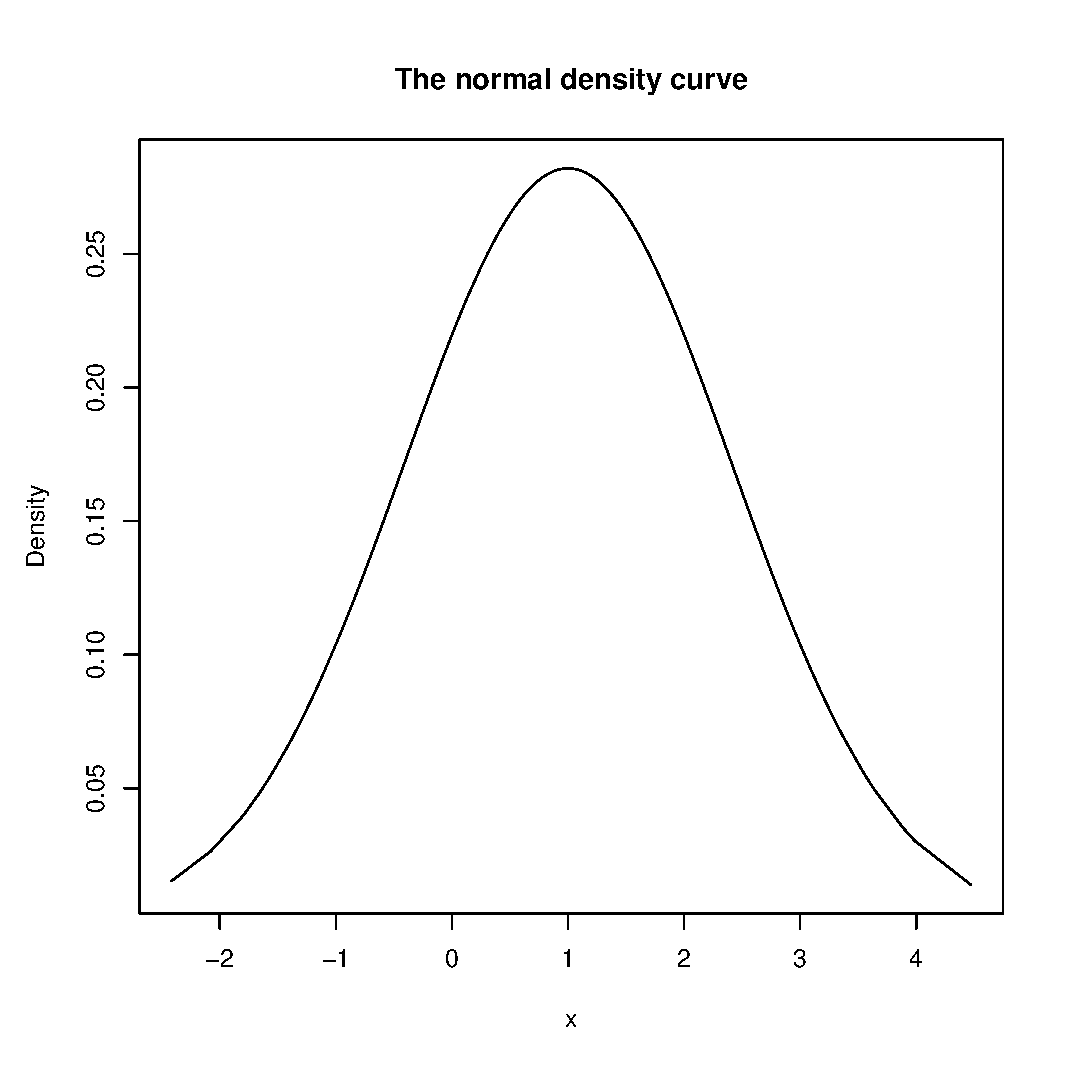
\includegraphics[width=0.6\textwidth]{NormCur.eps}
      \caption{The normal density curve $\mathcal{N}(\mu=1,\sigma^2=2)$}
      \label{fig:normcurve}
    \end{figure} 


  \item Calculate the  corresponding cumulative densities $P(x\leq X_i)=\int_{-\infty}^{X_i}P(x,
    \mu=1,\sigma^2=2)\mathrm{d}x$ and name it as \texttt{myPNormVec}.


  \item Plot the cumulative density curve where the x-axis should be
    \texttt{myRNormVec} and the y-axis should be the corresponding cumulated
    densities. Modify the axis labels so the final output looks like Figure
    \ref{fig:normcdfcurve} [Hint: again you need to sort \texttt{myRNormVec}
    firstly and then order \texttt{myPNormVec} accordingly.]

    \begin{figure}
      \centering
      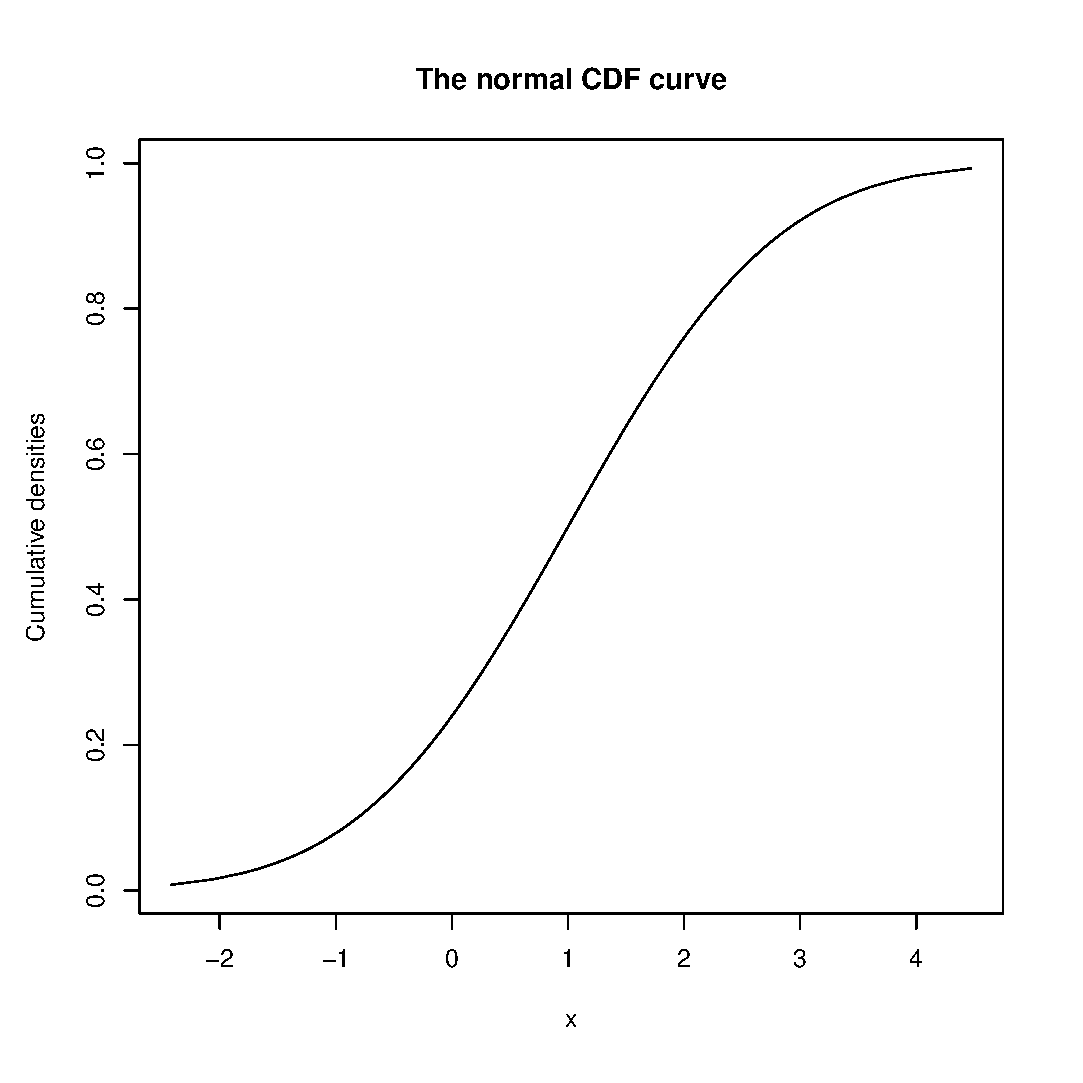
\includegraphics[width=0.6\textwidth]{NormCDFCur.eps}
      \caption{The normal CDF curve $\mathcal{N}(\mu=1,\sigma^2=2)$}
      \label{fig:normcdfcurve}
    \end{figure}
 
  \item Use the command \texttt{dev.copy2pdf(file="NormCDFCurve.pdf")} to save your
    current figure into pdf format.

  \item Calculate the quantiles for the vector \texttt{myPNormVec} which is
    from $\mathcal{N}(\mu=1,\sigma^2=2)$ and compare your results with
    \texttt{myRNormVec}.

  \item \textbf{Extra:} Can you compute these probabilities: $P(x>X_i)$ and
    $P(0<x<X_i)$? [Hint: $P(x>X_i) = 1 - P(x \leq X_i)$ and $P(0<x<X_i)= 1- P(x
    \geq X_i)- P(x \leq 0)$.] 
  \end{enumerate}


\section{}
\begin{enumerate}
\item Load the Apple and Google datasets from \textbf{computer lab 3} and name
  it as \texttt{Apple} and \texttt{Google} respectively. Store the variable (column)
  \texttt{High} from \texttt{Apple} in a new vector named \texttt{appleHigh}.
  
\item Calculate the mean and variance for \texttt{appleHigh}. Normalize the vector
  so that the mean and the variance are zero and one for the  new vector and
  name it as \texttt{appleHighStd}.

\item Perform a \emph{t} test where the null hypothesis is: The mean value of
  \texttt{appleHighStd} is 1. Answer the following questions [Hint: ?\texttt{t.test}] 

  \begin{enumerate}
  \item What confidence level did you use?
  \item What is the corresponding confidence interval?
  \item Can you reject the null hypothesis?
  \end{enumerate}
\end{enumerate}

\section{}
We continues to use the Apple and Google datasets.
\begin{enumerate}
\item Pick up the \texttt{Close} columns from the two datasets and name them as
  \texttt{appleClose} and \texttt{googleClose} respectively. Create a new
  variable
\begin{verbatim}
time <- length(appleClose):1
\end{verbatim}
which indicates the time id for the stock prices for the two companies.

\item Make a scatter plot of the \texttt{appleClose} agaist \texttt{time}
. Add ``time'' as the x-axis label, ``Prices'' as the
y-axis label and ``Plot for stock prices'' as the main title. 

\item Redo \textbf{4.2} but change the plot type into lines instead of
  scatters. Change the color of the line as blue and set \texttt{ylim} argument
  to \texttt{ylim = c(0, max(appleClose, googleClose))}.

\item Add a new line \texttt{googleClose} to the plot in \textbf{4.3} and set
  the line color as \texttt{red} [Hint: use \texttt{points()}]

\item Add a legend to the plot in \textbf{4.4} at a proper position to indicate
  different types of lines you have on the plot.

\item Save your plot into a file as png format. [Hint: \texttt{?savePlot}]

\item Make a histogram for \texttt{googleClose} and add a density curve on the
  histogram. Then use the following commands to save it as a jpeg file
 
\begin{verbatim}
dev.copy(jpeg,"GoogleClose-Hist.jpeg")
dev.off()
\end{verbatim}

\item Make a figure with 2-by-2 subplots. Pick four of your previous plots for
  Apple and Google data and fill them in the subplots (of course you have to
  redraw the plots). Save it as png format
  named \texttt{Stock-Apple-Google.png}.

\item \textbf{Extra:} Want to try more plot examples? See e.g.
  \url{http://gauss.stat.su.se/f/r/R_graphics.pdf} and
  \url{http://gauss.stat.su.se/f/r/R_graphics.R}
\end{enumerate}
 
\section{}
\begin{enumerate}
\item It is believed that the close price for the stock market may be affected
  by the highest stock price (e.g. the \texttt{High} data for the apple data),
  Make a simple regression model for the apple data with R where the response
  is \texttt{appleClose} and the explanatory variable is \texttt{appleHigh}, i.e 

  \begin{equation*}
    \mathtt{appleClose} = \hat \alpha + \hat \beta \mathtt{appleHigh} 
  \end{equation*}
  and save your regression model object as \texttt{appleModel}.

\item Study \texttt{appleModel} and answer the following questions.
  \begin{enumerate}
  \item What are the model coefficients?
    
  \item What are the confidence intervals for the regression coefficients?
 
  \item Make a histogram of the model residuals.

  \item Show the ANOVA table.

  \item Plot the model object.

  \end{enumerate}

\item The open price of the stock market can also be a factor that affects the
  close price. Extract the open price from the apple data and name it as
  \texttt{appleOpen}. Make a multiple regression 
 
  \begin{equation*}
    \mathtt{appleClose} = \hat \alpha + \hat \beta \mathtt{appleHigh} + \hat \gamma \mathtt{appleOpen} 
  \end{equation*}
  and save your regression model object as \texttt{appleModel2}.

 \item Study \texttt{appleModel2} and answer the queations in \textbf{5.2}. Did
   you get a better model?

 \item \textbf{Extra:} How can you make a linear regression without the
   intercept in R?

 \item The dataset \texttt{Apple} contains the stock prices for 1894 days. But
   you just want to use the recent 100 days (i.e. the first 100 rows). Explore
   the arguments of \texttt{lm()} to find how to implement that with \textbf{5.3}. 

 \item Actuary the three variables \texttt{open}, \texttt{low}, and
   \texttt{high} can possibly be the covariates of the model. But there are a
   lot of combinations. Use forward stepwise regression to find the best model
   starting with only an intercept and the scope model is the full model with
   all three covariates (use all the observations). 

 \item Did you end up with the same model when you use backward stepwise in
   \textbf{5.8}?

 \item \textbf{Extra:} You make the log transformation of the close price and treat the
   transformed data as the new response variable. Redo \textbf{5.7} with the
   transformed data.

\end{enumerate}


\end{document}